%===================================== CHAP 3 =================================

\chapter{Method}
This chapter will give an insight into why the research is needed and what method used conducting the research. Also, the chapter gives insight into the collection of data and the following analysis, as well as and who are the participants.

\section{Methodological Approach} \label{sec:purpose}
This study aims to understand the fundamental reason for the striking difference in labor productivity between the ICT-industry and CI. The research is, therefore, adopting a case study-strategy of a single-case object, in the CI in Norway. Utilizing a single-case study approach, preferably than multiple, will give a more in-depth look at the problem, rather than a thin description provided by the multiple-case study \cite{yin1993case}. This project, therefore, aims to examine a case using lean methodology, where digital tools are utilized to support both the method as well as cooperation and interaction between different actors. The project selected is the construction of the new Life Science Building, managed by Statsbygg \cite{statsbygg2019uio}. The problem of using case study is that it is hard to produce an generealized answer to a question. The aim of the research is not to obtain generalizable findings, but to explore the phenomenon. Moreover, the result of this research will give a knowledgeable background for the following master thesis. The intention is not to measure productivity, but rather understand why the difference occurs.

This study is related to the interpretivism paradigm — the use of empirical observation of the participants and a desire to identify how they act on the new software and methods used. Using interviews can lead to being subjective as all collection of data is done in interaction with the participants. This yields a qualitative collection of data. The purpose of this project thesis is to identify the problems worth exploring in the master thesis.

{\noindent \bf RQ1:} Why does the difference in LP between the ICT-industry and CI appear? \\
{\bf RQ2:} How does the difference appear in the LSB-project, which utilize both agile and digital tools?

\section{Data Collection}
\begin{figure}
    \begin{center}
        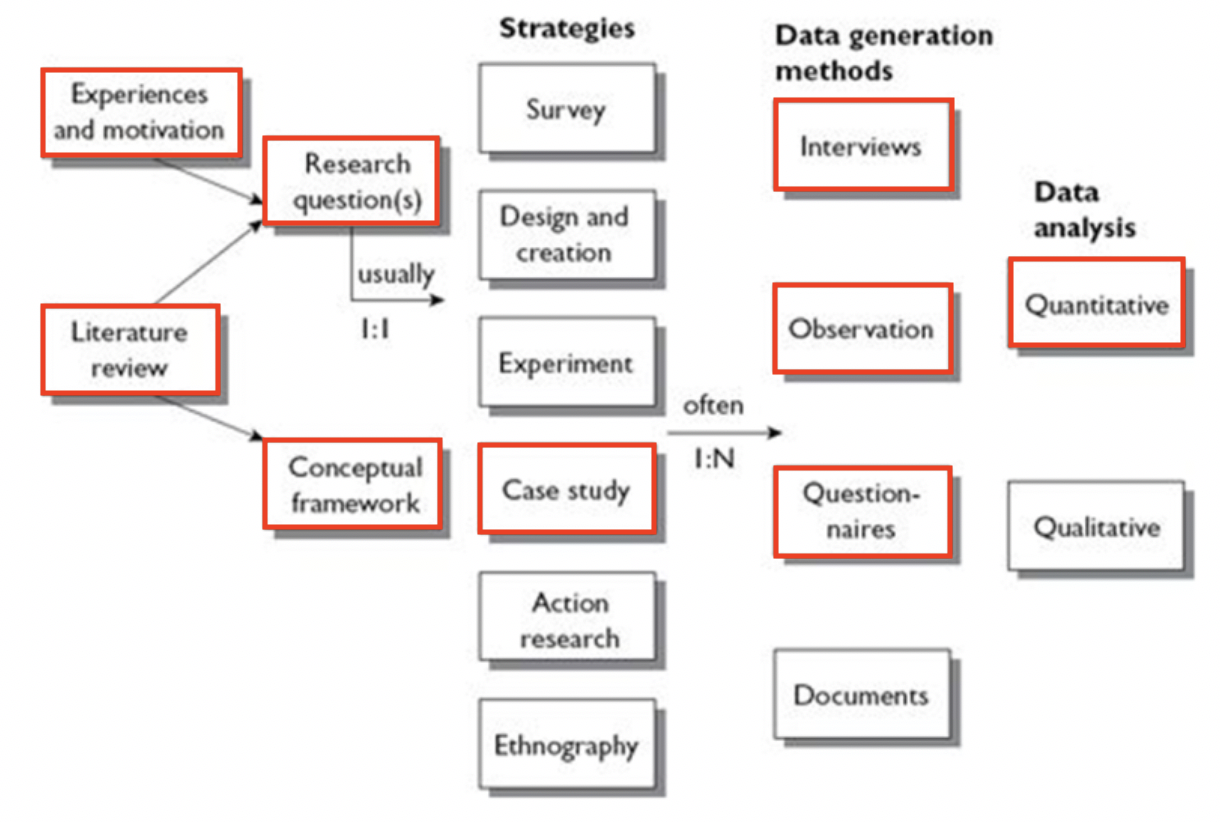
\includegraphics[width=0.75\textwidth]{fig/empirisk_studie.png}
        \caption{The research process used, marked with methods applied in the research.}
        \label{fig:research_process}
    \end{center}
\end{figure}

The project started with a literature review, providing a knowledgeable background as basis for the project. More importantly, the project consist of a minor empirical study, utilizing observation and interviews as data generators. The interviews was conducted with a semi-structured approach, with some standardized questions, listed in Appendix \ref{apx:interview_guide}, for every interview. The research process utilized in the projects can be seen in figure \ref{fig:research_process}.

The observations took place over two days, in the project office, where different meetings were observed. The observations were recorded with notes and transcribed after the observations. Except for the Digitalization meeting, the Researcher was not able to ask questions during the meeting.  Questions who came up was later answered by managers, or directly with participants, after the meetings. In addition to the observations and answering questions, talking to the managers and PLs, when on-site, gave valuable insight into how the project is run.

The interviews were done using Skype. With the consent of the participants, the sound was recorded. After the interview, the transcript was sent to the participants for them to approve. Both interviews took about 30-40 minutes. 

\begin{table}
    \begin{center}
        \begin{tabular}{p{.45\textwidth}p{.45\textwidth}}
        \toprule
        \textbf{Obervation} & \textbf{Meeting}       \\ \midrule
        1                   & Blackboard-meeting     \\
        2                   & Table-test meeting     \\
        3                   & Digitalization-meeting \\
        4                   & BIM and dRofus introduction \\
        Total observations  & \multicolumn{1}{r}{4}  \\ \bottomrule
        \end{tabular}
        \caption{List of observations conducted in the project thesis.}
        \label{tab:observations}
    \end{center}
\end{table}

\section{Participants}
The project researcher, Morten Bujordet, is involved in the project, creating the plans, and conducting the research.
	 
Supervising the project is Eric Monteiro. Monteiro is contributing with experience in research in the implementation and use of new digital tools in large scale, as welle as complex organizations. 

Furthermore, Statsbygg, as the manager, has an interest in the project: giving access to the participants in the study. With Patrick Stormo Hjerpseth as the point of contact.
	 
In the research, the actors using the digital software in the project design will be an aim for the data collection. All personal information gathered will, safely, be stored in a GDPR-compliant Cloud Service, served by NTNU. In the final report, no personal information will be published, and all actors in the data collection will be anonymized. The participants chosen for the interviews are key personnel leading the project of the managing organization. The list of interviewees can be seen in table \ref{tab:paticipants}. 

\begin{table}
    \begin{center}
        \begin{tabular}{p{0.3\textwidth}p{.3\textwidth}p{.3\textwidth}}
        \toprule
        \textbf{Interviewee} & \textbf{Function}          & \textbf{Gender} \\ \midrule
        1                    & Assistant Project Director \& Project Manager & Male            \\
        2                    & Assistant Project Manager  & Male            \\
        Total interviews     & \multicolumn{2}{r}{2}                        \\ \bottomrule
        \end{tabular}
        \caption{Overview over interviews in the project thesis.}
        \label{tab:paticipants}
    \end{center}
\end{table}

\section{Data Analysis}
The analysis started by transcribing the interviews and observations. Furthermore, utilizing a thematic analysis approach, the data was coded into three themes; (1) interaction, (2) responsibility, and (3) lack of understanding. Each theme was examined, gaining an understanding of participants' perceptions. Moreover, the results were analyzed using the literature review, comparing the subjects with previous experience found in literature. 

The thematic analysis was done by first transcribing the interviews. When the interviewees accepted the transcribed interviews, the process of coding was conducted. The coding of the text resulted in the three themes mentioned. Table \ref{tab:thematic-analysis} shows how the project combined codes into themes. As one can see, the code \textit{Contracts} is to be found both in the \textit{Interaction} and the \textit{Decision Making} theme. The connection was very present and found as an underlaying reason for them both. It was after the definition of the themes the analysis took place, and then the conclusion of the findings. Moreover, the same themes were used analyzing the observations and when comparing with the literature review.

% Please add the following required packages to your document preamble:
% \usepackage{booktabs}
\begin{table}[]
    \begin{center}
        \begin{tabular}{p{0.45\textwidth}p{.45\textwidth}}
        \toprule
        \textbf{Codes}        & \textbf{Themes} \\ \midrule
        \begin{itemize}
            \item Lack of understanding
            \item Wrong use
            \item New methods
        \end{itemize}         & \vspace{0.4mm}Ignorance       \\ 
        \begin{itemize}
            \item Responsibility?
            \item Agrements
            \item Protecting
            \item Contracts
        \end{itemize}         & \vspace{0.4mm}Decision Making \\
        \begin{itemize}
            \item Communication
            \item Transparency
            \item Delegation
            \item Silo
            \item Contracts
        \end{itemize}         & \vspace{0.4mm}Interaction    
        \end{tabular}
        \caption{The process of turning of transcribed codes into different the three emerging themes.}
        \label{tab:thematic-analysis}
    \end{center}
\end{table}

\section{Evaluation of the Method}
The single-case study, as well as the use of unstructured interviews, produce results that cannot be generalized beyond the sample group. Still, they provide a more in-depth understanding of participants’ perceptions, motivations, and emotions. 

One can always argue that utilizing observations and interviews for data collection can tend to be subjective. However, the use of a qualitative approach is best when wanting to describe, contextualize, and gain an in-depth insight into specific concepts or phenomena, which was the case in this empirical study. Furthermore, the number of interviewees and observations was quite poor. The result produced can, thus, be questioned. Though the result of the study does not stand for itself, it is identifying the problems worth further exploration in the master thesis, which is achieved, and therefore, more acceptable.

\cleardoublepage